\documentclass[herrin-thesis.tex]{subfiles}
\begin{document}

\chapter{Data Collection and Processing}
\label{ch:data}

\section{Signal Readout}
\label{sec:data_signal_readout}
\begin{figure}
\centering
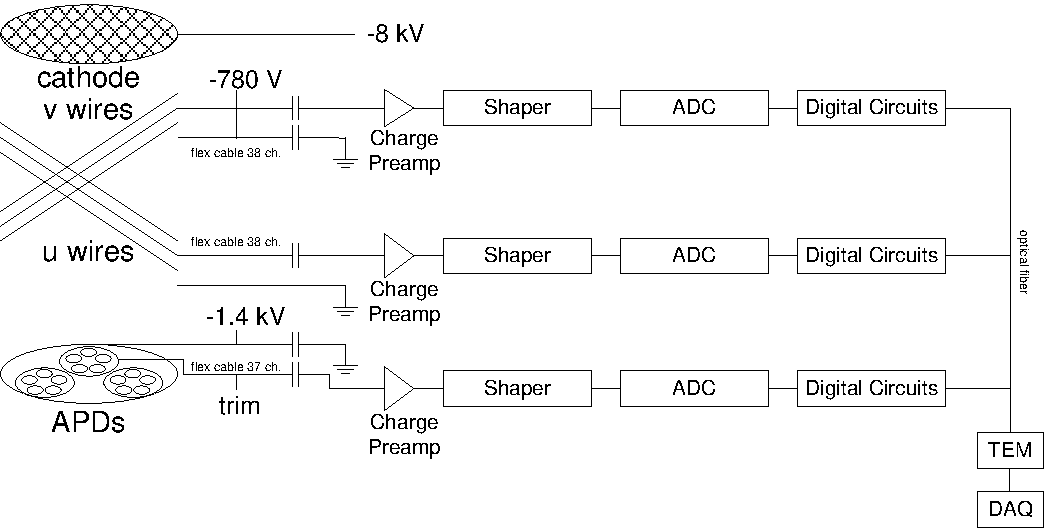
\includegraphics[width=\textwidth]{./figures/data_simplified_electronics.pdf}
\caption[The EXO-200 electronics]{A simplified schematic of the EXO-200 electronics. The ionization and scintillation signals are read out through long flex cables. The signals are shaped, digitized, and passed to the Trigger Event Module (TEM), which passes the data to the DAQ computers for recording when signals are detected.}
\label{fig:data_simplified_electronics}
\end{figure}

\begin{table}[tbp]
\centering
\caption[Electronic shaping times]{The shaping times for the signal readouts in EXO-200.}
\label{tab:data_shaping_times}
\begin{tabular}{l c @{\hskip 20pt} c c c @{\hskip 20pt} c c c}\toprule
							&&						\multicolumn{6}{c}{Stage Type}													\\\cmidrule{3-8}
	Channel Type				&&	\multicolumn{2}{c}{Integration (\si{\micro\s})}	&&	\multicolumn{3}{c}{Differentiation (\si{\micro\s})}				\\\midrule
	APDs					&&	3				&		3			&&	10				&	10				&	300			\\
	\multirow{2}{*}{\(u\) wires}		&&	\multirow{2}{*}{1.5}	&	\multirow{2}{*}{1.5}	&&	\multirow{2}{*}{40}	&	\multirow{2}{*}{40}	& 	measured 	\\
							&&					&					&&					&					& 	(nominally 60)	\\
	\(v\) wires					&&	3				&		3			&&	10				&	10				&	60			\\\bottomrule
\end{tabular}
\end{table}

\Cref{fig:data_simplified_electronics} shows a simplified schematic for the EXO-200 electronics. The APD signals and the ionization inductions and collection signals are read out through long flex cables. The long cables separate the electronics from the TPC, removing the need for cryogenic and low-radioactivity components. After passing through a preamplifier, the signals are fed through shaping circuits and are then digitized at a rate of \SI{1}{\MHz}. The shaping circuits consist of two integrators followed by two differentiators and one final differentiator on the charge preamp. \Cref{tab:data_shaping_times} summarizes the time constants.  The transfer functions of these shapers determine the waveform of a physical signal (ionization or scintillation). In order to improve energy resolution, the final stage differentiation times for the \(u\) wire channels are measured by analyzing the response to charge injected from a capacitor.

After digitization, the Trigger Event Module (TEM) monitors the signals to select interesting events. Due to the low radioactive backgrounds in EXO-200, and the relatively slow rate of \twonu, this trigger is extremely permissive. It is 100\% efficient at triggering on events that deposit more that \todo{Look up} in the liquid xenon. The average trigger rate during routine data taking is approximately \SI{8}{\mHz}. Additionally, the trigger is forced to fire every \SI{0.1}{\s} in order to ensure the DAQ system is correctly recording events and to provide a measurement of detector live time. When the trigger fires, the DAQ records a frame consisting of digitized waveforms for all channels \SI{\pm1024}{\micro\s} around the trigger time.

\section{Signal Reconstruction}
\subsection{Signal Finding}
Either scintillation or ionization signals may cause the trigger to fire. Since there is not a fixed time between the two types of signal, it is necessary to search for signals in the waveforms. This is done in a two stage process: first a matched filter technique searches for signals, and then a waveform unshaping technique refines the found signals. \Cref{fig:data_signal_finding} shows an example of this process.

\begin{figure}
	\centering
	\begin{subfigure}[t]{0.48\textwidth}
		\centering
		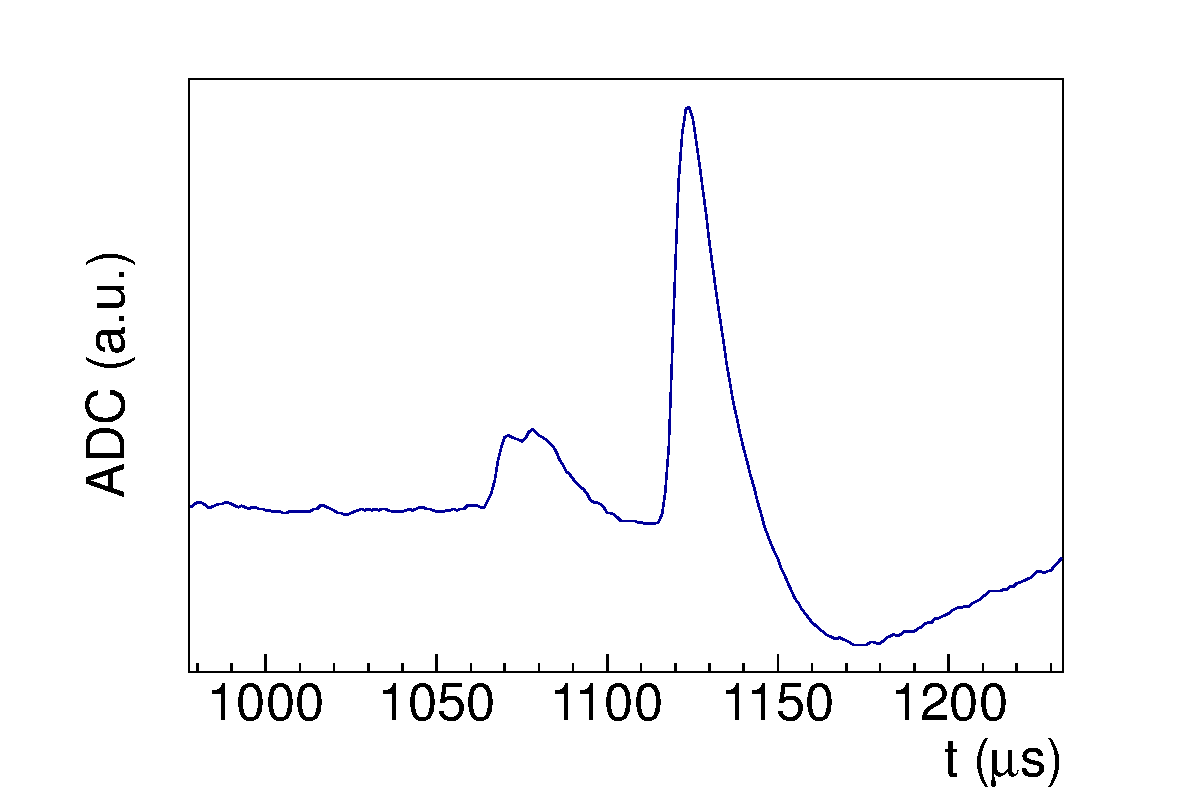
\includegraphics[width=\textwidth]{./plots/data_signal_finding_raw.pdf}
		\caption[Raw \(u\) wire waveform]{A raw \(u\) wire waveform showing two signals.}
		\label{fig:data_signal_finding_raw}
	\end{subfigure}\hfill%
	\begin{subfigure}[t]{0.48\textwidth}
		\centering
		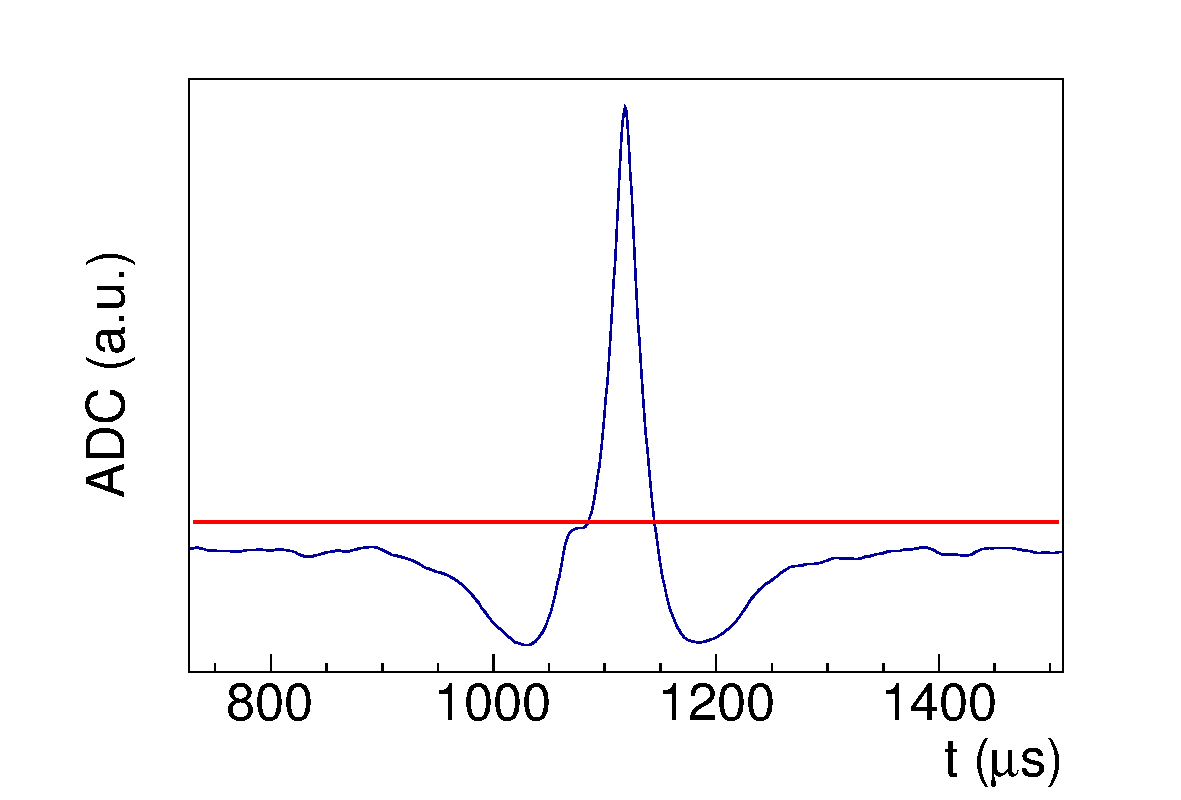
\includegraphics[width=\textwidth]{./plots/data_signal_finding_mf.pdf}
		\caption[Matched filter output]{The output of the matched filter with the threshold shown in red.}
		\label{fig:data_signal_finding_mf}
	\end{subfigure}
	\begin{subfigure}[t]{0.48\textwidth}
		\centering
		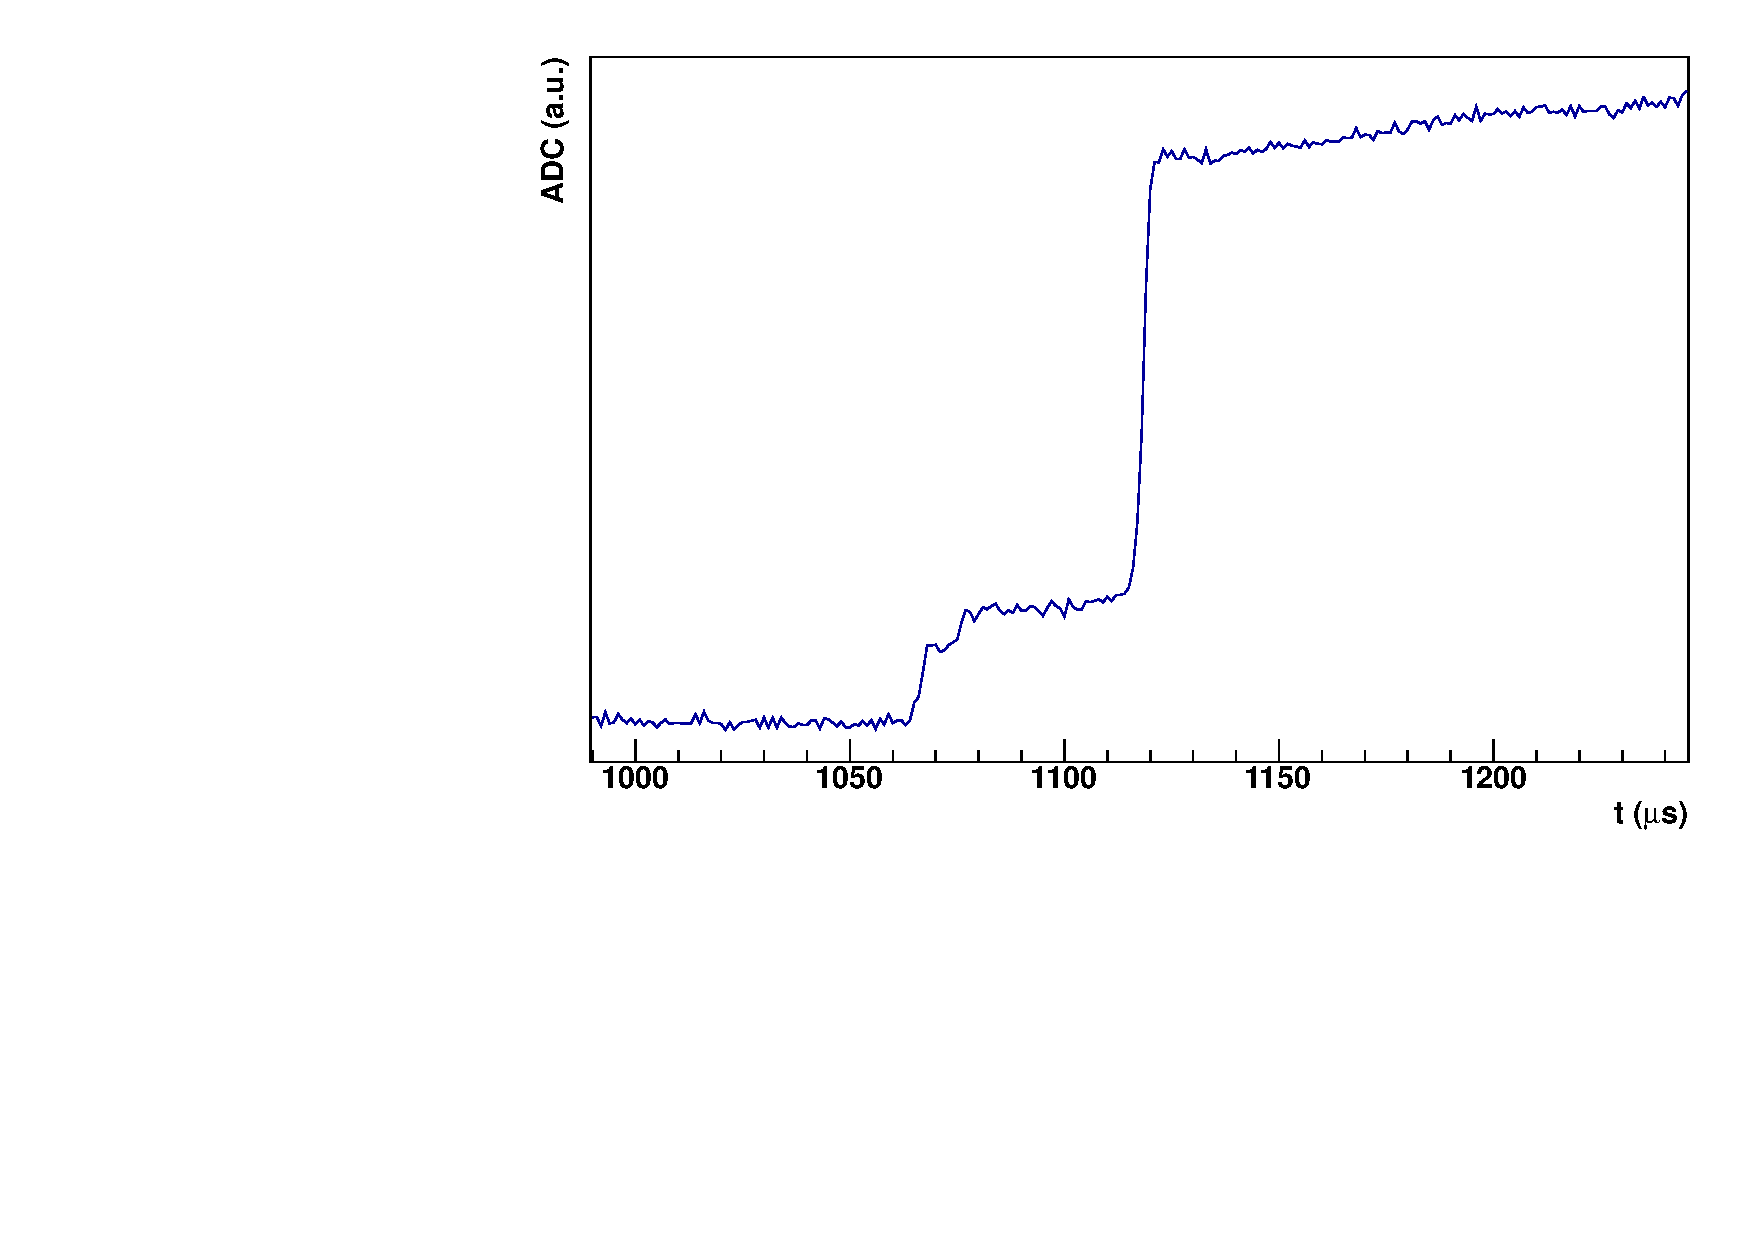
\includegraphics[width=\textwidth]{./plots/data_signal_finding_unshaped.pdf}
		\caption[Unshaped signals]{The `unshaped' signals.}
		\label{fig:data_signal_finding_unshaped}
	\end{subfigure}\hfill%
	\begin{subfigure}[t]{0.48\textwidth}
		\centering
		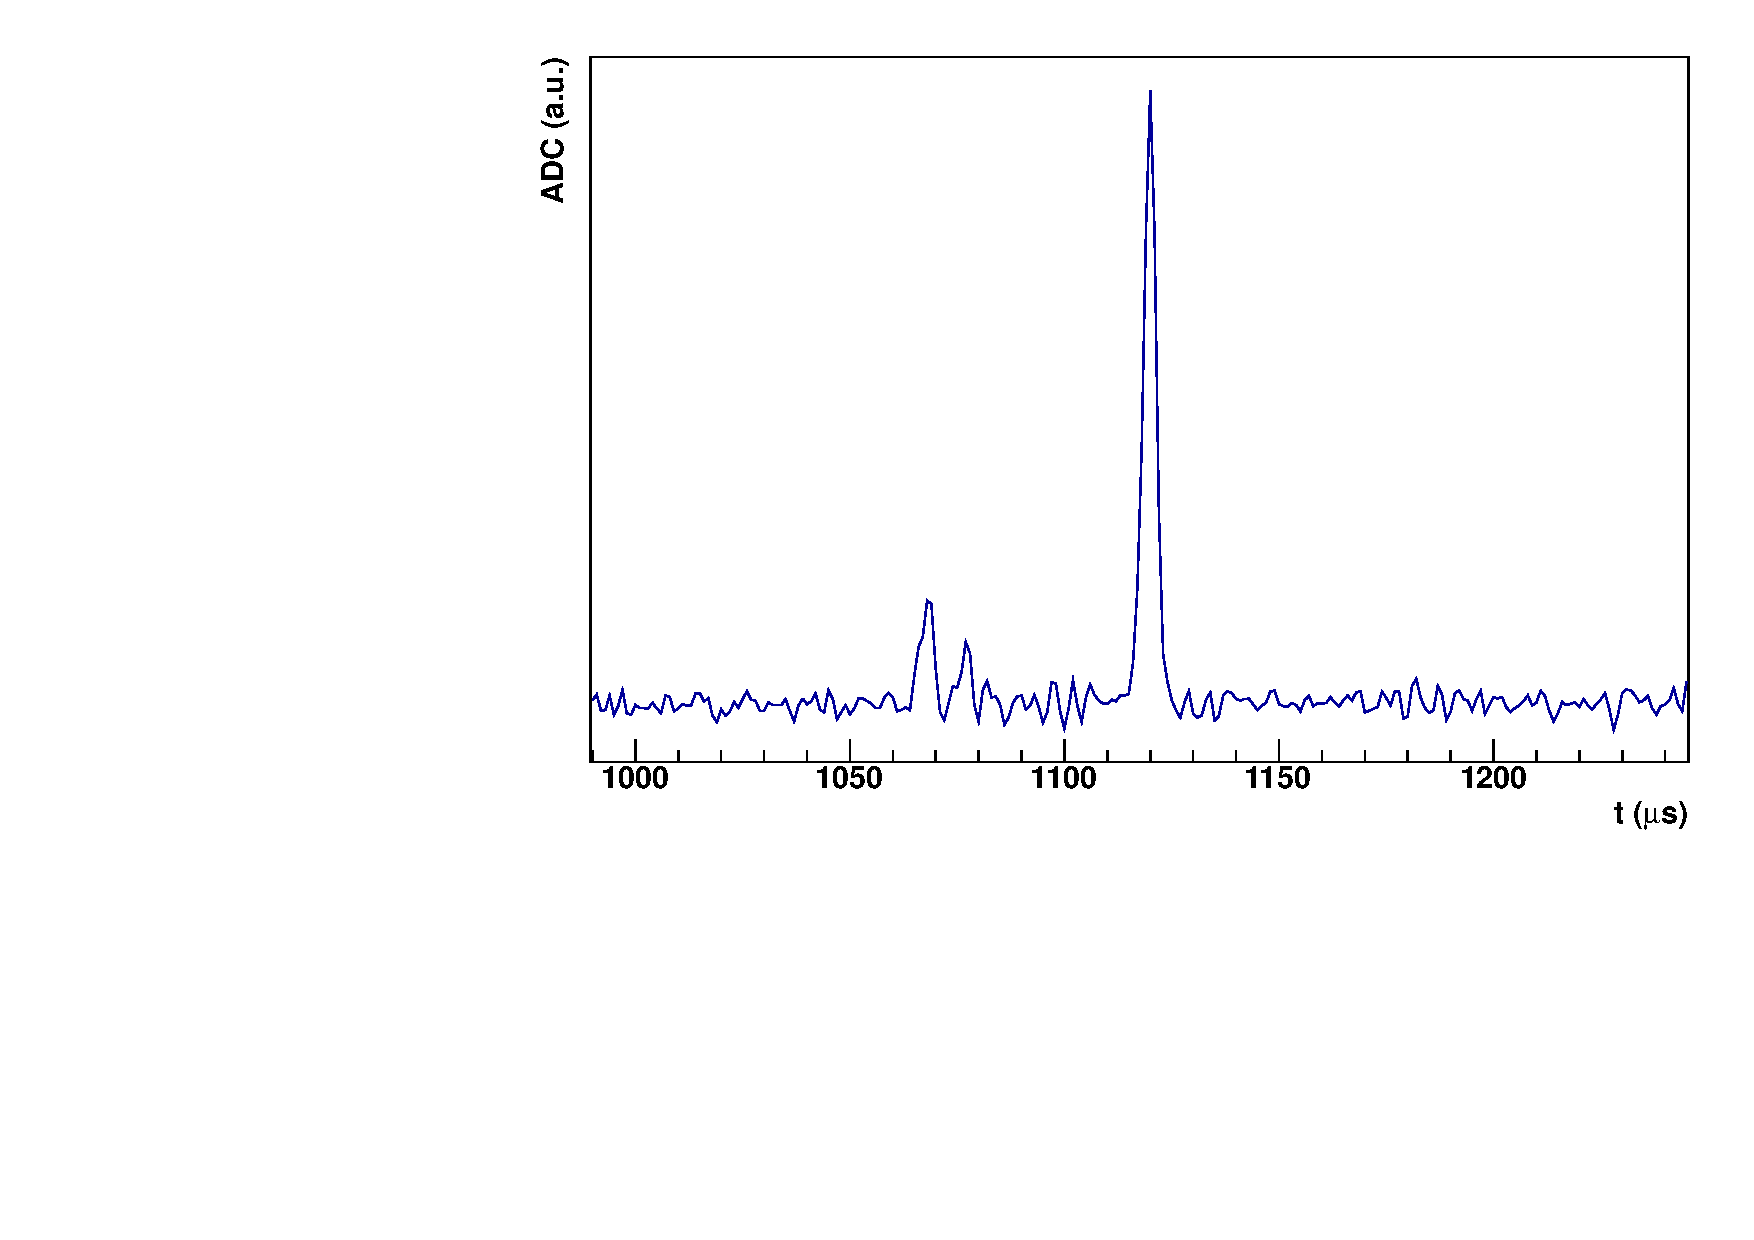
\includegraphics[width=\textwidth]{./plots/data_signal_finding_msf.pdf}
		\caption[Multiple signal finger output]{The output of a \SI{2}{\micro\s} triangular filter applied to the unshaped signals.}
		\label{fig:data_signal_finding_msf}
	\end{subfigure}
	\caption[The signal-finding process]{An example of finding signals on a \(u\) wire waveform.}
	\label{fig:data_signal_finding}
\end{figure}

The matched filter technique\cite{North:1963fk} convolves a time-reversed template signal with the waveform. Template signals are produced by passing a step function through the filters specified in \cref{tab:data_shaping_times}. This is done for individual channels for the \(u\) and \(v\) wires. For the APDs, the signals on the individual planes are summed and this technique is applied to these two sum signals. A threshold is determined by calculating the mean absolute deviation (MAD) of the waveform from its baseline. Parts of the waveform exceeding \((3\sqrt{\pi/2})\times\text{MAD}\) are excluded and the MAD is recalculated. A signal is found if the filter output exceeds 5 (4) times this final MAD for the wire (APD) signals. \Cref{fig:data_signal_finding_raw,fig:data_signal_finding_mf} show an example of this process.

While the matched filter is good at identifying that there was a signal on a wire, a refined analysis is needed to identify if multiple signals occurred in a short period of time. As \cref{fig:data_signal_finding_raw} shows, the matched filter only finds one signal when two are clearly visible. To find other signals, a \SI{256}{\micro\s} portion of the raw waveform is unshaped (by convolving the signal with the inverse transfer function of the shapers), then reshaped with a \SI{2}{\micro\s} triangular filter. Peaks in the output correspond to distinct signals. Finding multiple signals aids in discriminating against Compton-scattering \(\gamma\) ray backgrounds.

\subsection{Signal Parameter Extraction}
Once signals have been identified in a waveform, information about their energies and times are extracted by fitting a template waveforms (determined by the shaping times in \cref{tab:data_shaping_times}) to the waveforms. This is done by minimizing the \(\chi^2\) statistic formed by comparing the baseline-subtracted waveform to the template waveform. Signals that fit to similar times are combined. Signals that fit to small amplitudes or have large errors on the fit amplitude are removed. Minimization is repeated until no more signals need to be combined or removed. This is done on the individual \(u\) and \(v\) wire channels, and on the two plane sum APD signals.

Signals that are collected on a \(u\) wire channel can induce signals in neighboring channels. These induction signals could be mistaken for collection signals. Induction signals are identified and removed by combining information from a number of metrics:
\begin{itemize}
\item The rise times and maximum-to-minimum times of the pulses in the waveforms are shorter for induction signals than collection signals.
\item The integrals of the unshaped waveforms are much larger for collection signals than induction signals.
\item Induction signals have a better \(\chi^2\) statistic when fit to a template induction signal than to a template collection signal.
\item Induction signals occur on channels that neighbor channels with very large collection signals (associated with events of \(\gtrsim\)~\SI{1}{\MeV}).
\end{itemize}

\subsection{Signal Clustering}
Once signals have been identified, signals of the same type may be bundled together:
\begin{itemize}
\item \(u\) wire signals: signals that are on neighboring channels and are within \SI{3.5}{\micro\s} of each other most likely came from the same energy deposition, and so are bundled together. This bundle is assigned the energy-weighted mean time and \(u\) position of the constituent signals.
\item \(v\) wire signals: induction effects from a single energy deposition may affect more than the nearest-neighbor channels. \(v\) wire signals are bundled together if \(|(t_{i} + (\SI{2.97}{\micro\s})\Delta v) - t_0|< \SI{4.5}{\micro\s}\), where \(t_0\) is the largest amplitude signal and \(\Delta v\) is the difference in channel number between the largest signal and signal \(i\). This is based on an empirical measurement that channels farther away from the event fit to earlier signal times. The resulting bundle is assigned the energy-weighted mean \(v\) position of the bundled signals and the time of the largest signal.
\item The sum APD plane signals are bundled together if they have times within \SI{6}{\micro\s} (based on the integration times for the shaping circuits). This bundle is assigned the energy-weighted mean time of the signals.
\end{itemize}

The \(z\) position of each \(u\) wire bundle is calculated using the time of the most recent scintillation bundle and the known drift velocity for ionization. If no scintillation bundle is found within the maximum physically possible drift time, the bundle is not assigned a \(z\) position. Later data quality cuts remove events that have more than one scintillation bundle within this time window, since the \(z\) position becomes ambiguous.

Finally, \(u\) signal bundles are paired with \(v\) signal bundles. For each possible pairing, a likelihood is computed used 3 PDFs:
\begin{itemize}
\item After correcting for the known drift velocity between the anodes, the distribution of two paired \(u\) and \(v\) bundle times is a Gaussian centered around 0, with the standard deviation determined by the timing resolution of \SI{1}{\micro\s}.
\item The relationship between \(u\) and \(v\) signal magnitudes has been studied. Once the magnitudes of the bundles have been appropriately scaled, the distribution of their differences is again Gaussian, smeared by the energy resolution.
\item Not all \(u\) and \(v\) wire channels cross. If a pairing would cause the signal to be outside the hexagon containing the wires, the likelihood is penalized. The perpendicular distance to the edge of this hexagon is calculated. The penalty is the likelihood to be that distance away from the mean of a Gaussian distribution with standard deviation \SI{4.5}{\mm} (half the wire pitch).
\end{itemize}

The paired \(u\) and \(v\) bundles provide a 2D transverse position for the event. Since the wires do not cross at right angles, this position is translated to a \((x, y)\) position. The \(+y\) direction is vertically upward, the \(+x\) direction is away from the cryostat door, and \(+z\) is along the TPC axis and chosen to make the coordinate system right-handed. The position \((x, y, z) = (0, 0, 0)\) is defined to be the center of the detector, which is the center of the cathode.

\section{Corrections}
In order to have good energy resolution, events of the same energy should be reconstructed with the same energy, regardless of where in the detector they originated or on which channels the signals were collected. In order to achieve this, a number of corrections are applied to correct for both gain and positional variation. They are detailed below.

\subsection{Wire Gain Corrections}
\begin{figure}
	\begin{subfigure}[t]{0.48\textwidth}
		\centering
		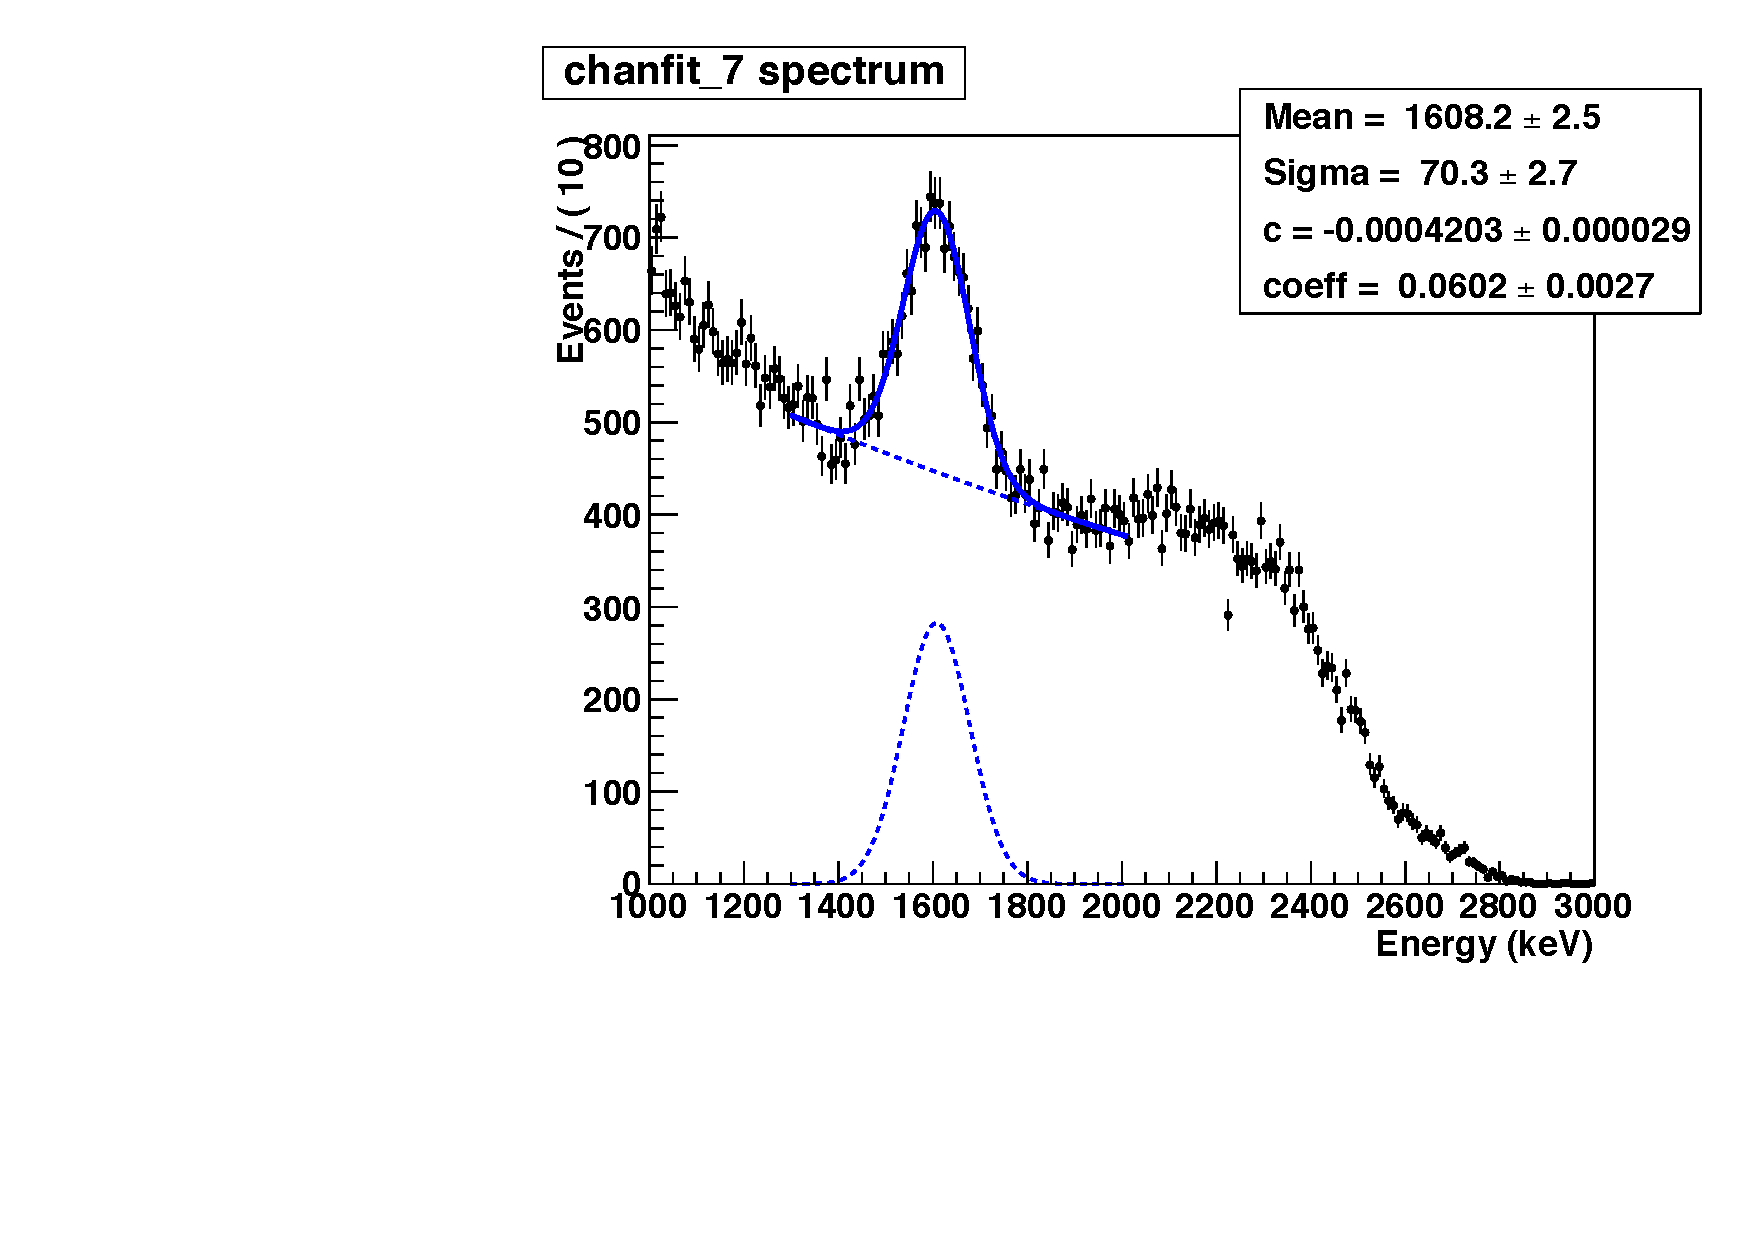
\includegraphics[width=\textwidth]{./plots/data_wiregain_pp07.pdf}
	\end{subfigure}\hfill%
	\begin{subfigure}[t]{0.48\textwidth}
		\centering
		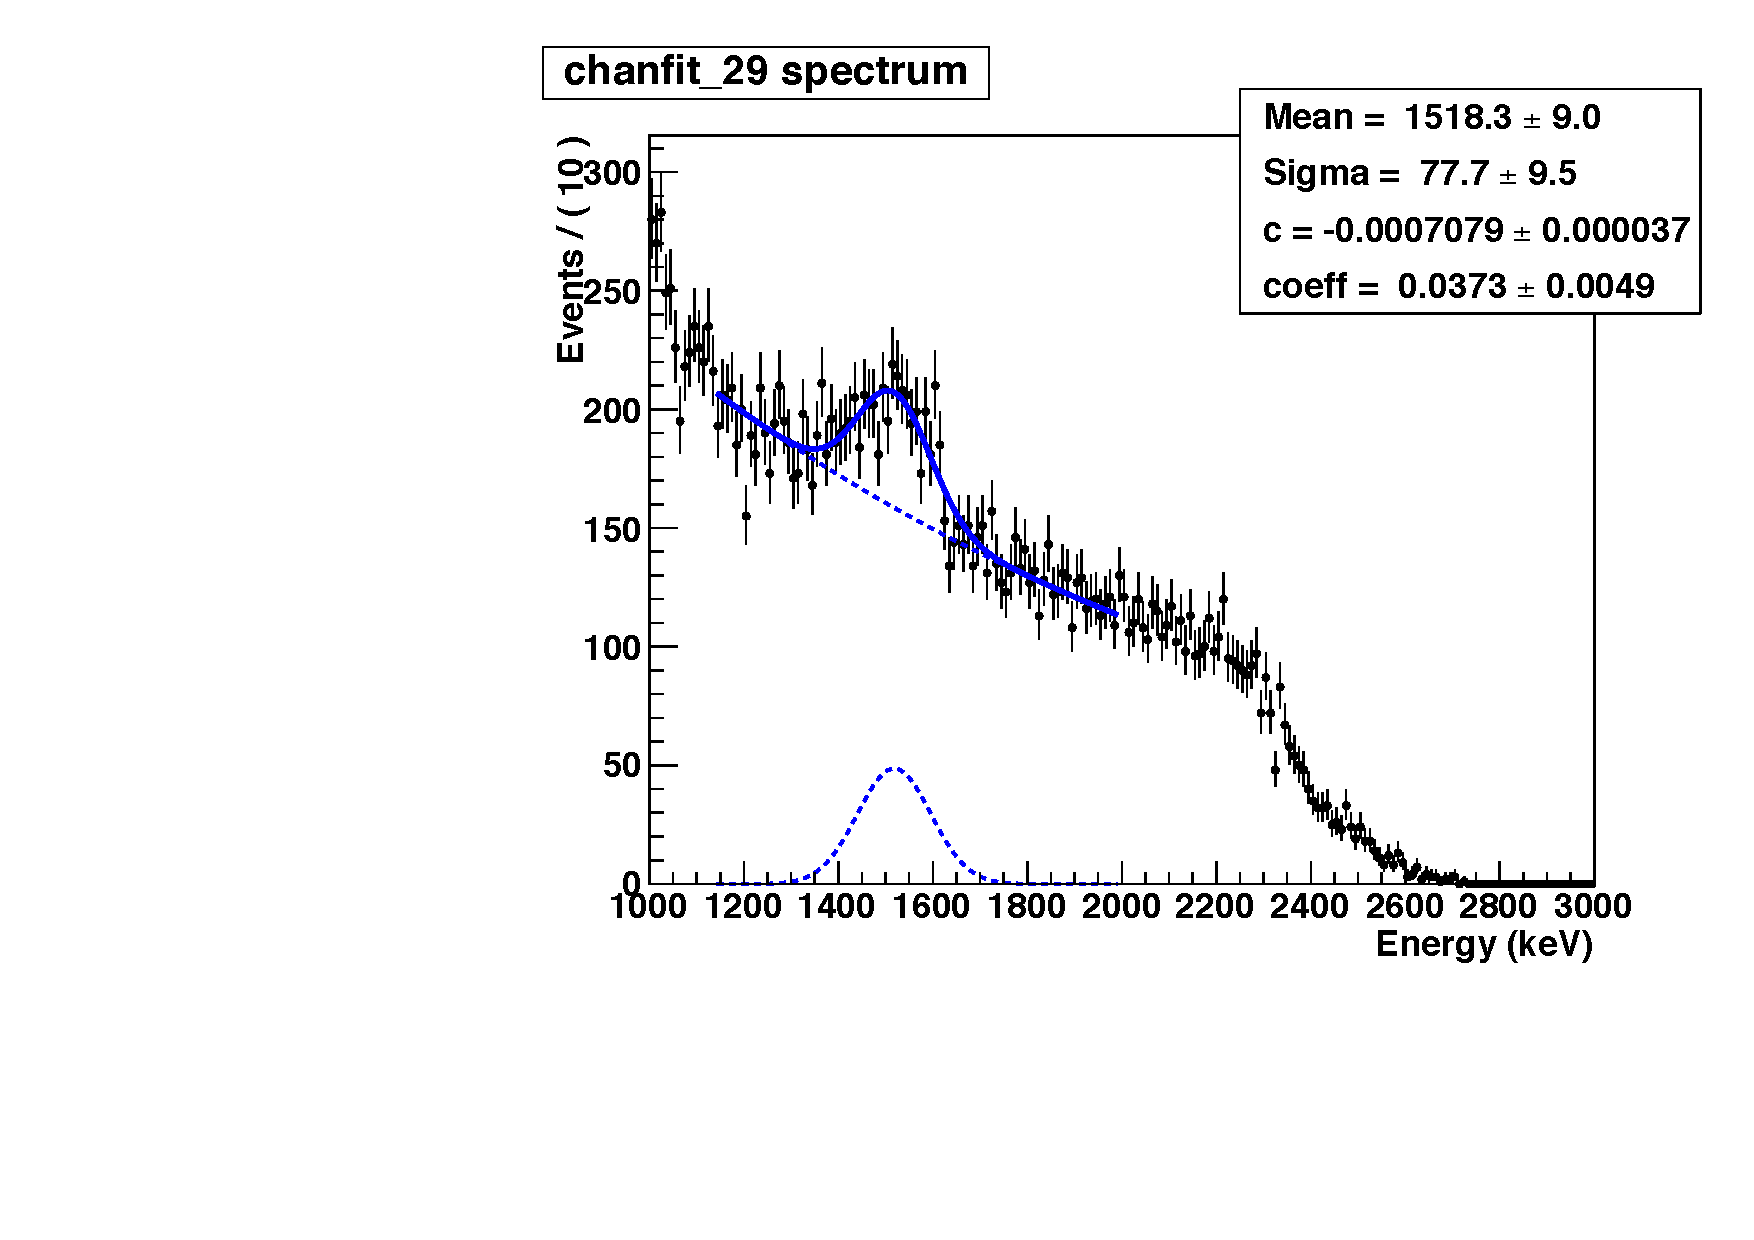
\includegraphics[width=\textwidth]{./plots/data_wiregain_pp29.pdf}
	\end{subfigure}
	\caption[The pair-production peak on individual \(u\) wire channels]{The \SI{1593}{\keV} pair-production peak shown on two different, uncorrected \(u\) wire channels. A Gaussian peak with an exponential background matches the observed spectrum well, and the mean obtained from the fit is then used to correct for channel-to-channel variations.}
	\label{fig:data_wiregain_pp}
\end{figure}

Minute differences in the components that read out each \(u\) wire channel can cause channel-to-channel variation in their responses. In order to address this, data from \thorium{228} calibration runs is used. The \SI{2615}{\keV} \(\gamma\) ray can produce an electron-positron pair with combined energy \SI{1593}{\keV}. Since the electron and positron deposit their energy in a small volume, this peak is clearly visible on individual wire channels. A scaling factor for each channel is determined by fitting these peaks scaling so that it occurs at the same value for each channel. \Cref{fig:data_wiregain_pp} shows examples for two channels.

Environmental conditions can also cause the response to shift over time. To address this, each channel has a capacitor that can inject a known amount of charge. These charge injections are done \about{} daily and used to measure the shaping time for the charge preamp (see \cref{sec:data_signal_readout}), but can also be used to measure the time variation of each individual channel. The time variation is tracked, and applied as a very small correction on top of the channel-to-channel correction.

\subsection{Shielding Grid Correction}
When ionization is created in a TPC, the positively charged ions move more slowly than the much less massive electrons. These positive ions can induce a signal on the collection wires opposite the collection signal. The measured signal will be reduced. For events far from the anode, the induction wire grid shields the collection wires from this effect. However, closer to the anode, the shielding grid is not perfect\cite{Bunemann:1949kx}, and so this effect must be corrected for.\todo{Fill in final details, whatever gets decided on.}

\subsection{Electron Lifetime Correction}
Ionization drifting in the TPC is attenuated by attachment to electronegative impurities. For uniformly distributed impurities, this results in an exponentially decreasing signal as a function of drift time, and the corresponding time constant is the ``electron lifetime''. This effect can be measured by measuring the attenuation of a known signal (as during a radioactive source calibration). This measurement is then used to correct unknown signals. \Cref{ch:electronlifetime} details the measurement of the electron lifetime and correction.

\subsection{Light Collection Correction}
While trim voltages are applied to the APDs to try to achieve a uniform response, there is still some variation in the gain from channel to channel. Additionally, there is geometric variation in the amount of scintillation light actually reaching the APDs due to shadowing from the wire planes, imperfect reflection off of the walls, and other effects. Using radioactive source calibration runs, the overall response from both of these factors can be mapped out and corrected for. \Cref{app:lightmap} details this correction.

\section{Calibration}

\section{Data Quality Cuts}

\end{document}
